\documentclass[serif,mathserif]{beamer}
\usepackage{etex}
\usepackage{amsmath, amsfonts, epsfig, xspace}
\usepackage{algorithm,algorithmic}
\usepackage{pstricks,pst-node}
\usepackage{multimedia}
\usepackage[normal,tight,center]{subfigure}
\usepackage[english]{babel}
\usepackage{beamerthemesplit}
\usepackage[utf8]{inputenc}

\usepackage{amsmath, amsthm, amssymb}
\usepackage{multicol}
\usepackage{textpos}

\newcommand{\itab}[1]{\hspace{0em}\rlap{#1}}
\newcommand{\tab}[1]{\hspace{.2\textwidth}\rlap{#1}}

\newcommand{\tip}{{\bf T}}
\newcommand{\al}{\mathcal{AL}}
\newcommand{\alc}{\mathcal{ALC}}
\newcommand{\alct}{\mathcal{ALC}+\tip}
\newcommand{\alctmin}{\mathcal{ALC}+\tip_{\mbox{\scriptsize \em min}}}
\newcommand{\nuovoc}{\mathrel{{\mathcal{T}\!\mathcal{AB}}}_{min}^{\mathcal{ALC}+\mbox{\scriptsize $\tip$}}}
\newcommand{\primo}{\mathrel{{\mathcal{T}\!\mathcal{AB}}}_{\scriptsize PH 1}^{\mathcal{ALC}+\mbox{\scriptsize $\tip$}}}
\newcommand{\secondo}{\mathrel{{\mathcal{T}\!\mathcal{AB}}}_{\scriptsize PH 2}^{\mathcal{ALC}+\mbox{\scriptsize $\tip$}}}
\newcommand{\LT}{\mathcal{L_\tip}}


\newcommand\Wider[2][3em]{%
\makebox[\linewidth][c]{%
  \begin{minipage}{\dimexpr\textwidth+#1\relax}
  \raggedright#2
  \end{minipage}%
  }%
}

\setlength{\subfigcapskip}{-.5em}
\usetheme{Frankfurt}
\usecolortheme{default}
%\usecolortheme{whale}
\beamertemplatenavigationsymbolsempty

\renewcommand{\familydefault}{\sfdefault}
%\usepackage{helvet}

\usepackage{tikz}
\usepackage{pgfgantt}

%%%%%%%%%%%%% TITLE %%%%%%%%%%%%%%

\author[Luca Violanti]{Candidato: Luca Violanti\\Relatore: Gian Luca Pozzato\\Controrelatore: Alberto Martelli}

\title[DysToPic\hspace{2em}\insertframenumber/\inserttotalframenumber]{\textbf{DysToPic}: a \\ Distributed Theorem Prover\\for non--monotonic\\Description Logics}

\date{10 Ottobre 2014} %leave out for today's date to be insterted

\institute{Università degli studi di Torino - Dipartimento di Informatica}

\usepackage{graphicx}
\begin{document}

\maketitle

\begin{frame}
	\frametitle{Description Logics (DLs)}
	
	\begin{block}{Description Logics}
	\begin{itemize}
	\item Decidable fragment of first order logic
  	\item Used for knowledge representation
		\begin{itemize}
			\item Ontologies (e.g. BabelNet, WordNet, Gene Ontology)
			\item Semantic web (e.g. OWL)
			\item Biomedical informatics (e.g. SNOMED CT, GALEN)
		\end{itemize}
	\end{itemize}
	\end{block}
	
\end{frame}

\begin{frame}
  \frametitle{Description Logics (DLs)}
  A DL defines a domain in terms of
  \begin{itemize}
  \item Individuals
  \item Concepts
  \item Roles
  \end{itemize}
\end{frame}

\begin{frame}
	\frametitle{Knowledge Base}
	\begin{block}{Intensional part: Terminological Box (\textbf{TBox})}
	E.g.:
		\begin{itemize}
		\item $Penguin \sqsubseteq Bird$\\
		\item $Bird \sqsubseteq Animal$\\
		\item $Cat \sqsubseteq Animal$\\[0.4cm]
		\end{itemize}
	\end{block}		
	\begin{block}{Extensional part: Assertional Box (\textbf{ABox})}
	E.g.:
		\begin{itemize}
		\item $Bird(tweety)$\\
		\item $Cat(sylvester)$
		\item $Hates(sylvester, tweety)$
		\end{itemize}
	\end{block}
\end{frame}

\begin{frame}
	\frametitle{Knowledge Base: example}

	A model of the previous KB
	\begin{figure}[htp]
	\centering
	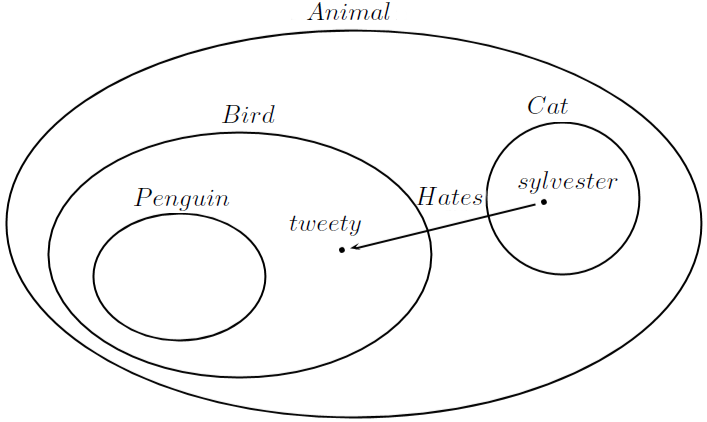
\includegraphics[scale=0.30]{img/diagram1_5.png}
	\end{figure}
\end{frame}

\begin{frame}
	\frametitle{Inference: query entailment}
	\begin{block}{Query entailment}
	A formula $F$ entails from a $KB$ if every model of such KB is also a model of $F$. We write $KB \models F$.
	\end{block}
	
	E.g., from the previous example:
	\begin{itemize}
		\item $KB \models Penguin \sqsubseteq Animal$
		\item $KB \not\models Penguin(sylvester)$
	\end{itemize}
\end{frame}

\begin{frame}
	\frametitle{Limits of the ``basic'' DLs}
	They do not allow:
	\begin{itemize}
	\item \textbf{typical} properties
	\item \textbf{defeasible inheritance}
%	\item per gestire l'ereditarietà defeasible richiedono meccanismi di ragionamento non--monotoni
%	
%	Es: - vari esempi (default, circumscription, ...)
	\end{itemize}
\end{frame}

\begin{frame}
	\frametitle{Solution: \tip}
	
	\begin{block}{Typicality}
	A typicality operator is added (\tip) to the existing DL.\\
	Therefore we can model concepts as:
	\begin{itemize}
	\item $\tip(C)$, i.e. the \textbf{typical instances} of concept C\\
	\end{itemize}
	\end{block}
	
	E.g.:
	\begin{itemize}
	\item $\tip(Bird) \sqsubseteq FlyingAnimal$
	\end{itemize}
\end{frame}

\begin{frame}
	\frametitle{$\alct$: syntax}
	
	\small
	Given an alphabet of concept names $\mathcal{C}$, role names $\mathcal{R}$, and individual constants $\mathcal{O}$, we can define the language $\mathcal{L}$ of $\alct$:
	
	\normalsize
	\begin{block}{Constants}
	any $a \in \mathcal{O}$ is a constant of $\mathcal{L}$.
	\end{block}
	\begin{block}{Concepts}
	if $C, D \in \mathcal{L}$ and $R \in \mathcal{R}$, then
	\begin{multicols}{2}
		\begin{itemize}
		\item $A \in \mathcal{C}$
		\item $\top$
		\item $\bot$
		\item $C\sqcap D$
		\item $C \sqcup D$
		\item $\neg C$
		\item $\forall R.C$
		\item $\exists R.C$
		\item \alert{$\tip(C)$}
		\end{itemize}
	\end{multicols}
	are concepts of $\mathcal{L}$.
	\end{block}
\end{frame}

\begin{frame}
	\frametitle{$\alct$: semantics}
	\begin{block}{Models}
	A model $\mathcal{M} = \langle \Delta, \mathcal{I}, < \rangle$ consists of
	\begin{itemize}
	\item $\Delta$, a non--empty set (domain)
	\item the preference relation $<$, an irreflexive and transitive relation over $\Delta$ (domain)\\
	\footnotesize
	For all $S\subseteq \Delta$, for all $x \in S$, either $x \in Min_<(S)$ or $\exists y \in  Min_<(S)$ such that $y < x$.
	\normalsize
	%%FIXME: qui ci vorrebbe il discorso sulla smoothness condition	
	\item $\mathcal{I}$, an interpretation function which assigns:
		\begin{itemize}
		\item to each concept $C \in \mathcal{C}$, a set $C^{\mathcal{I}} \subseteq \Delta^{\mathcal{I}}$\\
		(the individuals of the domain which belong to $A$)
		\item to every atomic role $R$ a binary relation, $R^{\mathcal{I}} \subseteq \Delta^{\mathcal{I}} \times \Delta^{\mathcal{I}}$\\
		(a couple of elements of the domain)
		\item \alert{to every concept $\tip(C) \in \mathcal{C}$, a set $(\tip(C))^\mathcal{I} = Min_<(C^\mathcal{I}).$}
		\end{itemize}
	\end{itemize}
	\end{block}
\end{frame}

\begin{frame}
	\frametitle{$\alct$: semantics}
	\begin{block}{Preference as accessibility}
	Given a model $\mathcal{M}$, the definition of $\mathcal{I}$ is extended with
	\begin{itemize}
	\item $(\Box C)^\mathcal{I} = \{ x \in \Delta \ |\ for\ each\ y \in \Delta,\ if\ y<x\ then\ y \in C^\mathcal{I}\}$
	\end{itemize}
	Then we have that
	\begin{itemize}
	\item $x\in(\tip(C))^\mathcal{I} \iff x \in(C\sqcap \Box \neg C)^\mathcal{I}$
	\end{itemize}
	\end{block}
\end{frame}


\begin{frame}
	\frametitle{Example: $\alct$}
	\begin{figure}[h]
	\centering
	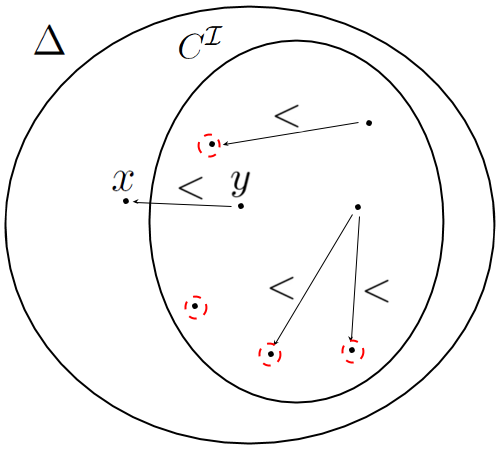
\includegraphics[scale=.30]{img/diagram1_9.png}
	\end{figure}

	\begin{itemize}
	\item the individuals which are $\tip(C)$ are highlighted
	\item $x$ is preferred to $y$, but it is not a $\tip(C)$ since it is not in $C^{\mathcal{I}}$
	\end{itemize}
\end{frame}

\begin{frame}
	\frametitle{Limit of $\alct$}
	It is \textbf{monotonic}!
	\begin{example}
	If we have a KB which contains
		\begin{itemize}
		\item $\tip(Bird) \sqsubseteq FlyingAnimal$
		\item $\tip(Bird \sqcap Penguin) \sqsubseteq \neg FlyingAnimal$
		\item $\tip(Bird \sqcap Penguin \sqcap \exists Owns.Jetpack) \sqsubseteq FlyingAnimal$
		\end{itemize}
		and		
		\begin{itemize}
		\item $\tip(Bird \sqcap Penguin \sqcap \exists Owns.Jetpack) (tux)$
		\end{itemize}
		\begin{multicols}{2}
		we can infer
		\begin{itemize}
		\item $FlyingAnimal(tux)$	
		\end{itemize}
		\vspace{2.1cm}
		
		\pause
		\begin{figure}[htp]
		\centering
		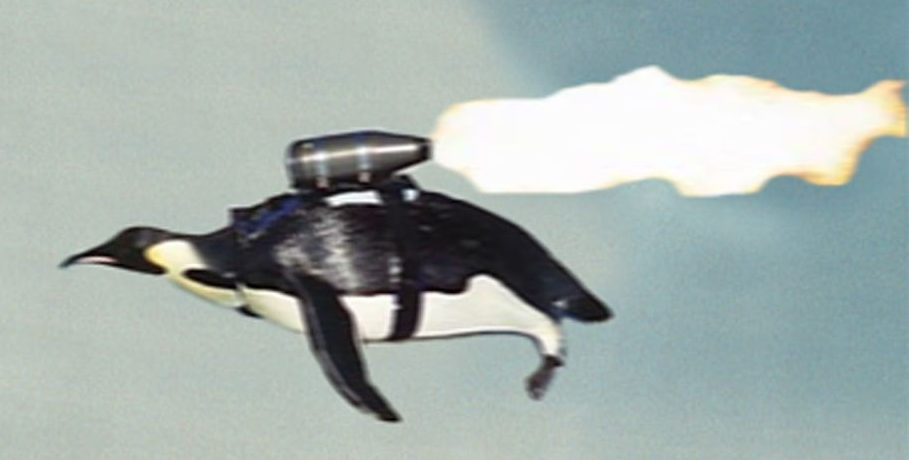
\includegraphics[scale=0.20]{img/penguin.png}
		\caption{}
		\label{}
		\end{figure}
		
		\end{multicols}
	\end{example}
\end{frame}

\begin{frame}
	\frametitle{Limit of $\alct$}
	\begin{example}
	But if we have a KB which contains
		\begin{itemize}
		\item $\tip(Bird) \sqsubseteq FlyingAnimal$
		\item $\tip(Bird \sqcap Penguin) \sqsubseteq \neg FlyingAnimal$
		\item $\tip(Bird \sqcap Penguin \sqcap \exists Owns.Jetpack) \sqsubseteq FlyingAnimal$
		\end{itemize}
		and		
		\begin{itemize}
		\item \alert{$(Bird \sqcap Penguin \sqcap \exists Owns.Jetpack) (tux)$}
		\end{itemize}
		we \textbf{cannot} infer
		\begin{itemize}
		\item $FlyingAnimal(tux)$	
		\end{itemize}	
	\end{example}
	
	We would like to infer that individuals \textbf{are typical instances} of the concepts they belong to, if this is consistent with the KB.
\end{frame}

%%FIXME: da aggiungere?
%% per gestire l'ereditarietà defeasible, in generale le DL richiedono meccanismi di ragionamento non--monotoni - citare solamente i vari esempi 	(default, circumscription, ...)

\begin{frame}
	\frametitle{Solution: $\alctmin$}
		The non--monotonic behaviour is obtained by restricting the attention to the \textbf{minimal} $\alct$ models
	\begin{block}{Non--monotonic semantics: Preference among models}
	Let us consider a finite set $\LT$ of concepts occurring in the KB.\\[0.2cm]
	A model $\mathcal{M}_1$ is preferred to $\mathcal{M}_2$ w.r.t. $\LT$ $(\mathcal{M}_1 <_\LT \mathcal{M}_2)$ if
		\begin{itemize}
		\item $\Delta_1 = \Delta_2$	
		\item for all $a$ in the ABox, $a^{\mathcal{I}_1} = a^{\mathcal{I}_2}$
		\item the set of $(x, \neg\Box\neg C)$ holding in $\mathcal{M}_1$ $\subset$ the set of $(x, \neg\Box\neg C)$ holding in $\mathcal{M}_2$ for $C \in \LT$
		\end{itemize}
	\end{block}
\end{frame}

\begin{frame}
	\frametitle{Solution: $\alctmin$}
	\begin{block}{Minimal entailment}
	A model $\mathcal{M}$ is \textbf{minimal} for a KB w.r.t. $\LT$ if
		\begin{itemize}
		\item $\mathcal{M}$ is a model of the KB
		\item there is no other model $\mathcal{N}$ of the KB s.t. $N <_\LT M$\\[0.5cm]
		\end{itemize}
		$F$ is \textbf{minimally entailed} from a KB w.r.t. $\LT$ \alert{$(KB \models_{min} F)$}\\[0.1cm]
		if $F$ holds in all the models of the KB which are minimal w.r.t. $\LT$
	\end{block}
\end{frame}


\begin{frame}
	\frametitle{The tableaux calculus $\nuovoc$}
	\begin{itemize}
	\item $\nuovoc$ is a tableaux calculus which 
	verifies whether a query entails from a KB (i.e. $KB \models_{min} F$ ?)\\[0.3cm]
	This is equivalent to stating that $F$ is verified in \textbf{all the minimal models} of the KB\\[0.3cm]
	\item To do so, the calculus tries to build a \textbf{minimal} model of $KB \cup \neg F$ (a \textbf{counterexample})
		\begin{itemize}
		\item if it fails, then the query entails from the KB
		\item otherwise it does not
		\end{itemize}
	\end{itemize}
\end{frame}

\begin{frame}
	\frametitle{The tableaux calculus $\nuovoc$}
 It is designed as a two--phase calculus:
		\begin{enumerate}
		\item first phase: $\primo$ 	
		\item second phase: $\secondo$	
		\end{enumerate}	

\end{frame}

\begin{frame}
	\frametitle{First phase: $\primo$}
	\begin{block}{$\primo$}
	Verifies whether $KB \cup \{\neg F\}$ is satisfiable in an $\alct$ model by generating \textbf{candidate models} $\mathcal{M}_i$
	\begin{itemize}
	\item the ones in which $F$ holds cannot be counterexamples, thus they are discarded
	\item a model $\mathcal{M}_i$ of $KB \cup \{\neg F\}$ in which $F$ does not hold, instead, \textbf{could be a counterexample}
	\end{itemize}
	\end{block}
\end{frame}

\begin{frame}
	\frametitle{Second phase: $\secondo$}
	\begin{block}{$\secondo$}
	For each candidate model $\mathcal{M}_i$, tries to build a model of the $KB$, $\mathcal{M}_j^{KB}$, which is preferred to $\mathcal{M}_i$
	\begin{itemize} 
	\item if every attempt of $\secondo$ fails on a candidate $\mathcal{M}_i$, $\mathcal{M}_i$ is the minimal model (i.e. the counterexample): $KB \not\models_{min} F$
	\item in case even a single $\mathcal{M}_j^{KB}$ is preferred to an $\mathcal{M}_i$, $\mathcal{M}_i$ is not the counterexample (but there could be another $\mathcal{M}_k$!)
	\item if every $\mathcal{M}_i$ has at least one corresponding $\mathcal{M}_j^{KB}$ so that $\mathcal{M}_j^{KB} <_\LT \mathcal{M}_i$, $KB \cup \neg F$ has no models, and $KB \models_{min} F$\\
	\end{itemize}
	\end{block}
\end{frame}


\begin{frame}
	\frametitle{First implementation of $\nuovoc$: \emph{PreDeLo}}
	Both phases had already been implemented in Prolog, and a theorem prover, called \emph{PreDeLo}, had been developed upon them

\begin{figure}[htp]
\centering
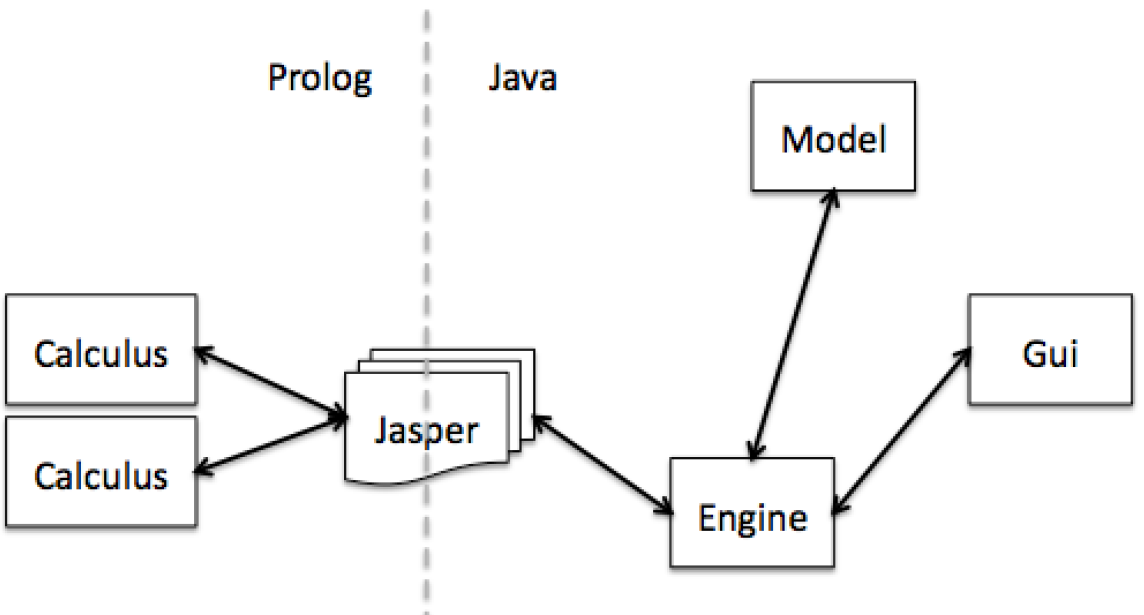
\includegraphics[scale=.30]{img/predelo.png}
\end{figure}
\end{frame}


\begin{frame}
\frametitle{Example: \emph{PreDeLo}}

Example of execution with the previous prover\\[0.2cm]

\begin{example}
	
	\begin{tikzpicture}
	\begin{ganttchart}[
		vgrid,
		canvas/.style={
			shape=rectangle,
			fill=white,
			draw=black}
		]{1}{17}
		\gantttitle{Sequential implementation}{17} \\
		\ganttbar[bar/.append style={fill= blue!30}]{\scriptsize Phase 1}{1}{1}
		\ganttbar[bar/.append style={fill= blue!30}]{}{5}{6}
		\ganttbar[bar/.append style={fill= blue!30}]{}{11}{12}
		\ganttbar[bar/.append style={fill= blue!30}]{}{16}{16}
		
		
		\ganttbar[inline,bar/.append style={fill= blue!30}]{\scriptsize $\mathcal{M}_1$}{1}{1}
		\ganttbar[inline,bar/.append style={fill= blue!30}]{\scriptsize $\mathcal{M}_2$}{5}{6}
		\ganttbar[inline,bar/.append style={fill= blue!30}]{\scriptsize $\mathcal{M}_3$}{11}{12}
		\ganttbar[inline,bar/.append style={fill= blue!30}]{\scriptsize $\mathcal{M}_4$}{16}{16}\\
		
		
		\ganttbar[bar/.append style={fill=red!30}]{\scriptsize Phase 2}{2}{4}
		\ganttbar[bar/.append style={fill=red!30}]{}{7}{10}
		\ganttbar[bar/.append style={fill=red!30}]{}{13}{15}
		\ganttbar[bar/.append style={fill=green!30}]{}{17}{17}
		
		\ganttbar[inline,bar/.append style={fill=red!30}]{\scriptsize $\mathcal{M}_1$}{2}{4}
		\ganttbar[inline,bar/.append style={fill=red!30}]{\scriptsize $\mathcal{M}_2$}{7}{10}
		\ganttbar[inline,bar/.append style={fill=red!30}]{\scriptsize $\mathcal{M}_3$}{13}{15}
		\ganttbar[inline,bar/.append style={fill=green!30}]{\scriptsize $\mathcal{M}_4$}{17}{17}
	\end{ganttchart}
	\end{tikzpicture}	
\end{example}

\end{frame}


\begin{frame}
\frametitle{A new implementation: \emph{DysToPic}}

We developed a \textbf{new theorem prover}, called \emph{DysToPic}, distributing the calculus, so that the two phases can be run in \textbf{parallel}\\[0.2cm]
\begin{block}{Architecture}
	We can identify the following ``actors'':
	\begin{itemize}
	\item client
	\item employer ($\primo$)
	\item worker ($\secondo$)
	\item repository
	\end{itemize} 
\end{block}
\end{frame}

\begin{frame}
	\frametitle{Implementation: architecture}
	\begin{figure}[htp]
\centering
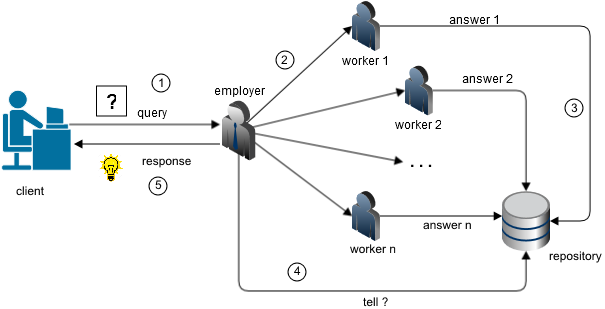
\includegraphics[scale=0.66]{img/DIAG_1.png}
\end{figure}
\end{frame}

\begin{frame}
\begin{example}
\frametitle{Implementation}
	
	\begin{tikzpicture}
	\begin{ganttchart}[
		vgrid,
		canvas/.style={
			shape=rectangle,
			fill=white,
			draw=black}
		]{1}{17}
		\gantttitle{Parallel implementation}{17} \\
		\ganttbar[bar/.append style={fill= blue!30}]{\scriptsize employer}{1}{1}
		\ganttbar[bar/.append style={fill= blue!30}]{}{2}{3}
		\ganttbar[bar/.append style={fill= blue!30}]{}{4}{5}
		\ganttbar[bar/.append style={fill= blue!30}]{}{6}{6}
		
		\ganttbar[inline,bar/.append style={fill= blue!30}]{\scriptsize $\mathcal{M}_1$}{1}{1}
		\ganttbar[inline,bar/.append style={fill= blue!30}]{\scriptsize $\mathcal{M}_2$}{2}{3}
		\ganttbar[inline,bar/.append style={fill= blue!30}]{\scriptsize $\mathcal{M}_3$}{4}{5}
		\ganttbar[inline,bar/.append style={fill= blue!30}]{\scriptsize $\mathcal{M}_4$}{6}{6}\\
		
		
		\ganttbar[bar/.append style={fill=red!30}]{\scriptsize worker1}{2}{4}
		\ganttbar[bar/.append style={fill=red!30}]{}{6}{8}
		
		\ganttbar[inline,bar/.append style={fill=red!30}]{\scriptsize $\mathcal{M}_1$}{2}{4}
		\ganttbar[inline,bar/.append style={fill=red!30}]{\scriptsize $\mathcal{M}_3$}{6}{8}\\
		
		
		\ganttbar[bar/.append style={fill=red!30}]{\scriptsize worker2}{4}{7}
		\ganttbar[bar/.append style={fill=green!30}]{}{8}{8}
		
		\ganttbar[inline,bar/.append style={fill=red!30}]{\scriptsize $\mathcal{M}_2$}{4}{7}
		\ganttbar[inline,bar/.append style={fill=green!30}]{\scriptsize $\mathcal{M}_4$}{8}{8}
	\end{ganttchart}
	\end{tikzpicture}	
\end{example}

\end{frame}

\begin{frame}
\frametitle{Implementation}

\begin{example}
	
	\begin{tikzpicture}
	\begin{ganttchart}[
		vgrid,
		canvas/.style={
			shape=rectangle,
			fill=white,
			draw=black}
		]{1}{17}
		\gantttitle{Parallel implementation}{17} \\
		\ganttbar[bar/.append style={fill= blue!30}]{\scriptsize employer}{1}{1}
		\ganttbar[bar/.append style={fill= blue!30}]{}{2}{3}
		\ganttbar[bar/.append style={fill= blue!30}]{}{4}{5}
		\ganttbar[bar/.append style={fill= blue!30}]{}{6}{6}
		
		\ganttbar[inline,bar/.append style={fill= blue!30}]{\scriptsize $\mathcal{M}_1$}{1}{1}
		\ganttbar[inline,bar/.append style={fill= blue!30}]{\scriptsize $\mathcal{M}_2$}{2}{3}
		\ganttbar[inline,bar/.append style={fill= blue!30}]{\scriptsize $\mathcal{M}_3$}{4}{5}
		\ganttbar[inline,bar/.append style={fill= blue!30}]{\scriptsize $\mathcal{M}_4$}{6}{6}\\
		
		
		\ganttbar[bar/.append style={fill=red!30}]{\scriptsize worker1}{2}{4}
		
		\ganttbar[inline,bar/.append style={fill=red!30}]{\scriptsize $\mathcal{M}_1$}{2}{4}\\
		
		
		\ganttbar[bar/.append style={fill=red!30}]{\scriptsize worker2}{4}{7}
		
		\ganttbar[inline,bar/.append style={fill=red!30}]{\scriptsize $\mathcal{M}_2$}{4}{7}\\
		
		
		\ganttbar[bar/.append style={fill=red!30}]{\scriptsize worker3}{6}{8}
		
		\ganttbar[inline,bar/.append style={fill=red!30}]{\scriptsize $\mathcal{M}_3$}{6}{8}
		\ganttbar[bar/.append style={fill=gray!30}]{}{8}{8}\\
		
		
		\ganttbar[bar/.append style={fill=green!30}]{\scriptsize worker4}{7}{7}
		
		\ganttbar[inline,bar/.append style={fill=green!30}]{\scriptsize $\mathcal{M}_4$}{7}{7}
				
	\end{ganttchart}
	\end{tikzpicture}	
\end{example}

\end{frame}



\begin{frame}
	\frametitle{Questions?}
	\Wider{
	\begin{figure}[htp]
	\centering
	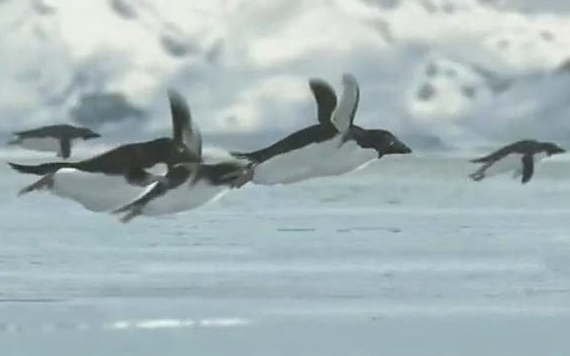
\includegraphics[scale=.5]{img/bbc.jpg}
	\end{figure}
	}
\end{frame}
\end{document}
